%%%%%%%%%%%%%%%%%%%%%%%%%%%%%%%%%%%%%%%%%
% University/School Laboratory Report
% LaTeX Template
% Version 3.0 (4/2/13)
%
% This template has been downloaded from:
% http://www.LaTeXTemplates.com
%
% Original author:
% Linux and Unix Users Group at Virginia Tech Wiki 
% (https://vtluug.org/wiki/Example_LaTeX_chem_lab_report)
%
% License:
% CC BY-NC-SA 3.0 (http://creativecommons.org/licenses/by-nc-sa/3.0/)
%
%%%%%%%%%%%%%%%%%%%%%%%%%%%%%%%%%%%%%%%%%

%----------------------------------------------------------------------------------------
%	PACKAGES AND DOCUMENT CONFIGURATIONS
%----------------------------------------------------------------------------------------

\documentclass{article}

%\usepackage{mhchem} % Package for chemical equation typesetting
%\usepackage{siunitx} % Provides the \SI{}{} command for typesetting SI units

\usepackage{graphicx} % Required for the inclusion of images
\usepackage[top=1in,bottom=1in,right=1in,left=1in]{geometry}% Set the margins

%Multiple column picture packages
\usepackage{caption}
\usepackage{subcaption}

%Add code formating
\usepackage{listings}
\lstset{tabsize=2}

%Define the style for VHDL
\lstdefinelanguage{VHDL}{
  morekeywords={
    library,use,all,entity,is,port,in,out,end,architecture,of,
    begin,and
  },
  morecomment=[l]--
}

%Give the VHDL code color
\usepackage{xcolor}
\colorlet{keyword}{blue!100!black!80}
\colorlet{comment}{green!90!black!90}
\lstdefinestyle{vhdl}{
  language     = VHDL,
  basicstyle   = \ttfamily,
  keywordstyle = \color{keyword}\bfseries,
  commentstyle = \color{comment}
}

\usepackage{amssymb}
\usepackage{amsmath}

%Highlight command
\usepackage{tikz}
\usepackage{xspace}
\usetikzlibrary{decorations.pathmorphing}
\newcommand\hl[1]{%
    \tikz[baseline,%
      decoration={random steps,amplitude=1pt,segment length=15pt},%
      outer sep=-15pt, inner sep = 0pt%
    ]%
   \node[decorate,rectangle,fill=yellow,anchor=text]{#1\xspace};%
}%

% Create the header and footer
\usepackage{fancyhdr}
\pagestyle{fancy}
\lhead{CprE 583}
\rhead{Blake Vermeer, Kris Hall, Rohit Zambre}
\renewcommand{\footrulewidth}{0.4pt}

\setlength\parindent{0pt} % Removes all indentation from paragraphs

\renewcommand{\labelenumi}{\alph{enumi}.} % Make numbering in the enumerate environment by letter rather than number (e.g. section 6)

%\usepackage{times} % Uncomment to use the Times New Roman font

%----------------------------------------------------------------------------------------
%	DOCUMENT INFORMATION
%----------------------------------------------------------------------------------------

\title{MP-1 Write-Up} % Add title here...

\author{Blake \textsc{Vermeer}\\
		Kris \textsc{Hall}\\
		Rohit \textsc{Zambre}} % Author name

\date{\today} % Date for the report

\begin{document}

\maketitle % Insert the title, author and date

\begin{center}
\begin{tabular}{l r}
Date Performed: & September 19, 2014 \\ % Date the experiment was performed
%Partners: & James Smith \\ % Partner names (optional)
Instructors: & Joseph Zambreno % Instructor/supervisor
\end{tabular}
\end{center}

% If you wish to include an abstract, uncomment the lines below
% \begin{abstract}
% Abstract text
% \end{abstract}


%----------------------------------------------------------------------------------------
%	SECTION 1
%----------------------------------------------------------------------------------------

\section{Objective}
In this lab we were introduced to the Xilinx tools and the lab environment setup. Also, we did some basic VHDL coding to manipulate a UART link.


\section{Initial Test}
After generating the bitfile, we uploaded the file to the Xilinx board. After running the program, LEDs 1 and 4 lit up and remained lit. I then connected to the Xilinx board over the serial link using minicom. The Xilinx board simply echoed back any data sent to it over the serial link. 


\section{Uppercase Conversion}
The TX\_driver signal is the input to the hardware module of MP1\_Top (TX\_driver is the output of the MP1\_top\_driver module that acts as the UART for the simulation) while the RX\_driver is the output of the hardware module of MP1\_top. In the screen-shot below, we can see that the RX\_driver signal is essentially a delay of the TX\_driver signal. RX\_driver echoes back the value of TX\_driver as soon as the 8 bits have been completely transferred.

	\begin{figure}[h]
		\begin{center}
			\includegraphics[scale=0.35]{../part3_files/MP1-Normal_Execution.png}
			\caption{Part 3 - Normal Execution waveform}
		\end{center}
	\end{figure}

The upper case conversion is implemented with the following code in the echo module:

\begin{center}

	\begin{lstlisting}[style=vhdl]
	
		if (data_in >= 97 and data_in <= 122) then
			data_out_reg <= (data_in - 32);		--convert to upper case
			
		else
			data_out_reg <= data_in;
		end if;
	
	\end{lstlisting}

\end{center}

We generated the bitfile of this design and were able to see the successful results in minicom. The small-case letters were echoed back as upper-case letters in minicom. The bitfile for this part is included with the submission.


\section{Exploring the Design}


	\begin{figure}[h]
		\begin{center}
			\includegraphics[scale=0.6]{../part4_files/part4_timing_diagram.png}
			\caption{Part 4 Timing Diagram}
		\end{center}
	\end{figure}


\section{Echo Delay}
The module works by taking in all signals sent between mmu\_uart\_top and process\_data and holding that information for one second, before sending it out to the respective components.

	\begin{figure}[h]
		\begin{center}
			\includegraphics[scale=0.6]{../part5_files/part5_block_diagram.png}
			\caption{Part 5 Block Diagram}
		\end{center}
	\end{figure}


\pagebreak


\section{In-Flight Calculations}
In this section, we modified the design so that it would echo back the sum of the previous two inputs if the last two characters entered we both 0 through 4. To do this we replaced the "echo" module with our own module called "num\_adder". Below is a block diagram for the design: \\


	\begin{figure}[h]
		\begin{center}
			\includegraphics[scale=0.55]{../block_diagrams/part_6_block_diagram_num_adder.png}
			\caption{Part 6 - Block Diagram}
		\end{center}
	\end{figure}

The design is fairly simple. It primarily consists of a state machine and some supporting logic. The state machine is responsible for detecting new data, storing this data in registers, detecting when the UART is free, and detecting the occurrence of two consecutive numbers between 0-4 and outputting their sum. There is a submodule contained within this design (num\_check) who's only job is to see if its two inputs are both 0-4 and return 1 if they are or 0 otherwise. Here is the state diagram for the state machine in "num\_adder": \\

	\begin{figure}[h]
		\begin{center}
			\includegraphics[scale=0.25]{../dot/Part-6_state_machine.png}
			\caption{NUM\_ADDER State Diagram}
		\end{center}
	\end{figure}

The state diagram is fairly straight forward. The module is normally waiting for new data to arrive. After new data arrives it waits for the UART module to be available to transmit the data. If the state machine received the signal from the "num\_check" module then it proceeds to wait for the UART module to become available again and then transmits the second byte of data. The only slightly strange state is the DELAY state. This was necessary since the UART module has a one clock cycle delay between receiving new data to transmit and the time when it unsets the TX\_busy\_n flag to signal that the UART is busy. 


\section{Changing the Baud Rate}
This section asked what changes would be necessary to change the baud rate of the module from 9600 to 38400. The well commented signals made that change fairly easy to find. In the "UART\_driver" module you would change the "ck\_div" input on the "UART\_1" instance to x"011E". This is based on the formula to find the baud rate given below:

	\begin{displaymath}
		baud\_rate = F(clk) / (ck\_div*3)
	\end{displaymath}

In our design, the base clock rate is 33MHz.

	\begin{displaymath}
		38400 = 33MHz / (ck\_div*3)
	\end{displaymath}
	
	\begin{displaymath}
		\boldsymbol{ck\_div = 286}
	\end{displaymath}







% If you have more than one objective, uncomment the below:
%\begin{description}
%\item[First Objective] \hfill \\
%Objective 1 text
%\item[Second Objective] \hfill \\
%Objective 2 text
%\end{description}

%\subsection{Definitions}
%\label{definitions}
%\begin{description}
%\item[Stoichiometry]
%The relationship between the relative quantities of substances taking part in a reaction or forming a compound, typically a ratio of whole integers.
%\item[Atomic mass]
%The mass of an atom of a chemical element expressed in atomic mass units. It is approximately equivalent to the number of protons and neutrons in the atom (the mass number) or to the average number allowing for the relative abundances of different isotopes. 
%\end{description} 
 
%----------------------------------------------------------------------------------------
%	SECTION 2
%----------------------------------------------------------------------------------------




%----------------------------------------------------------------------------------------
%	SECTION 4
%----------------------------------------------------------------------------------------
\section{Conclusion}
In this lab we were introduced to the tools we will be using throughout the semester. We were also reintroduced to VHDL coding and some of the best design practices when coding with VHDL.


%----------------------------------------------------------------------------------------
%	BIBLIOGRAPHY
%----------------------------------------------------------------------------------------
%\newpage

%\bibliographystyle{unsrt}

%\bibliography{sample}

%----------------------------------------------------------------------------------------


\end{document}